\documentclass[class=report, crop=false, 12pt,a4paper]{standalone}
\usepackage{enumitem}
\usepackage{graphicx}
\usepackage{float}
\usepackage{amsmath}
\usepackage{amssymb}
\usepackage{mathtools}
\usepackage{siunitx}
\usepackage{tikz}
\usepackage{commath}
\usepackage[a4paper,width=150mm,top=25mm,bottom=25mm]{geometry}
\begin{document}
\begin{center}
  19/10/2020
\end{center}
\section{First Order Systems}
All first order systems i.e. those with only $\frac{\dif x}{\dif t}$ take the following “standard” forms:
\begin{gather}
  \frac{X(s)}{Y(s)} = \frac{\alpha}{1+Ts} = \frac{\gamma}{1+\tau s}
\end{gather}
Where:
\begin{itemize}
  \item $\tau$, $\gamma$ is the \textbf{gain}
  \item T, $\tau$ is the \textbf{time constant}
\end{itemize}
This function is commonly known as an exponential time delay, or lag.
\subsection{Returning to the Time Domain}
To get the response of the system in the time domain we need to convert the transfer function from the Laplace domain. Tables of common inverse Laplace functions have already been created; all we need to do arrange our transfer function into one of these standard forms.
\begin{figure}[H]
  \centering
  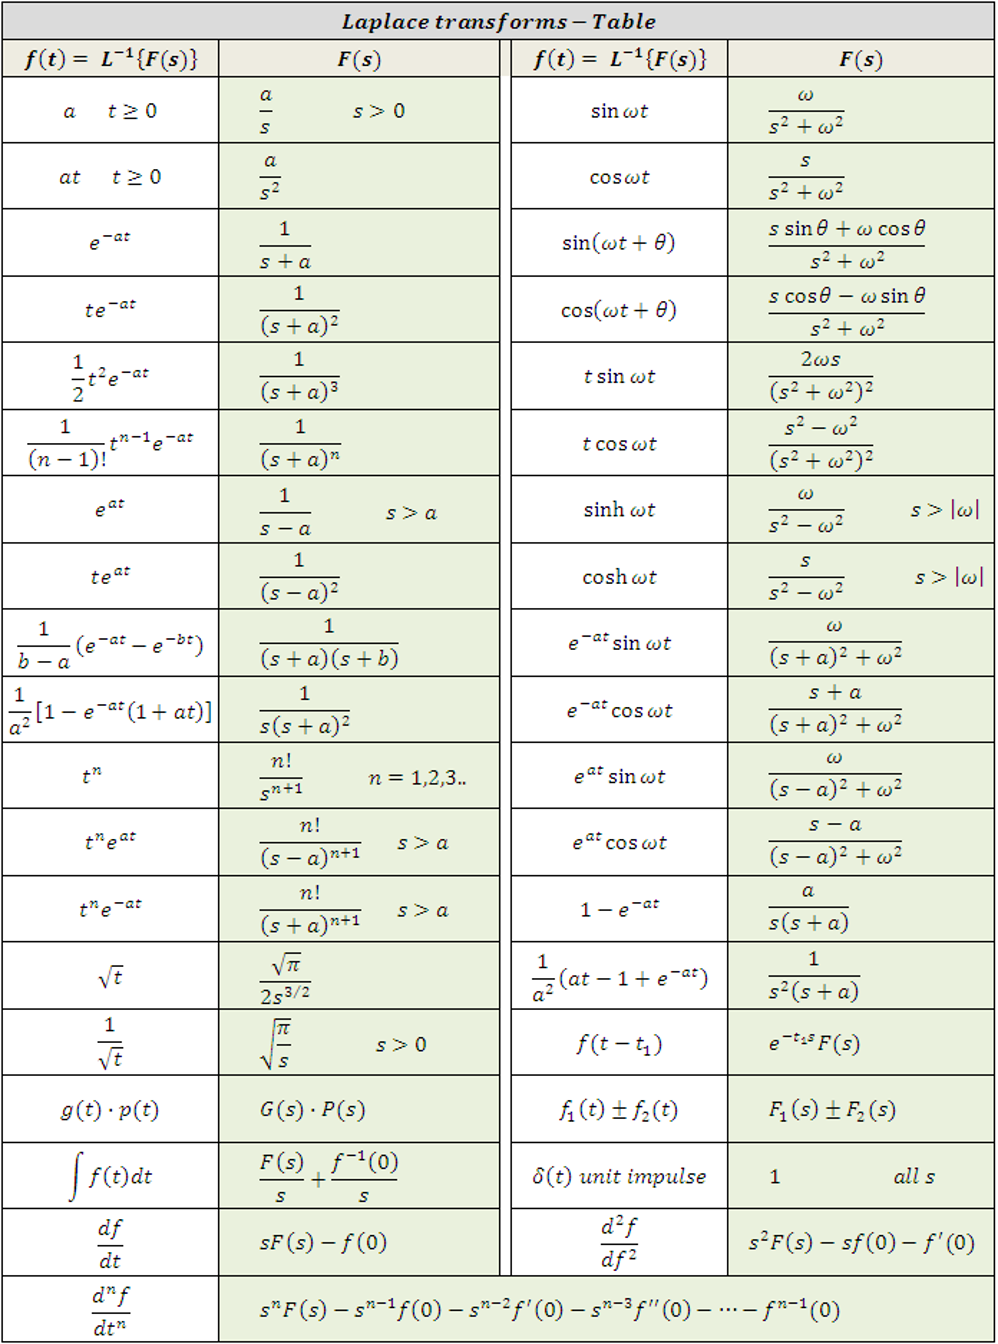
\includegraphics[width = 1 \textwidth]{../img/laplacetransformationtable.png}
  \caption{Laplace Transformation Table}
\end{figure}
\subsubsection*{Example: Parallel Spring \& Damper (Laplace Domain found previously)}
\begin{gather}
  \frac{X(s)}{Y(s)} = \frac{\alpha}{1+Ts} = \frac{\gamma}{1+\tau s}
\end{gather}
Looking at the table, we can find the relevant inverse function; in this case (3rd from the top):
\begin{gather}
  a = \frac{1}{\tau}
\end{gather}
Hence:
\begin{gather}
  \frac{X(s)}{Y(s)} = \frac{\frac{\gamma}{\tau}}{\frac{1}{\tau}+s} = \frac{\gamma}{\tau}\frac{1}{\frac{1}{\tau}+s} \\
  x(t) = L^{-1}\left\{\frac{\gamma}{\tau}\frac{1}{\frac{1}{\tau}+s}\right\} \\
  = \frac{\gamma}{\tau}L^{-1}\left\{\frac{1}{\frac{1}{\tau}+s}\right\} \\
  = \frac{\gamma}{\tau}e^{-\frac{t}{\tau}}
\end{gather}
This is an exponential decay – the only variable needed to define the system is the time constant. The gain merely scales the response.
\begin{figure}[H]
  \centering
  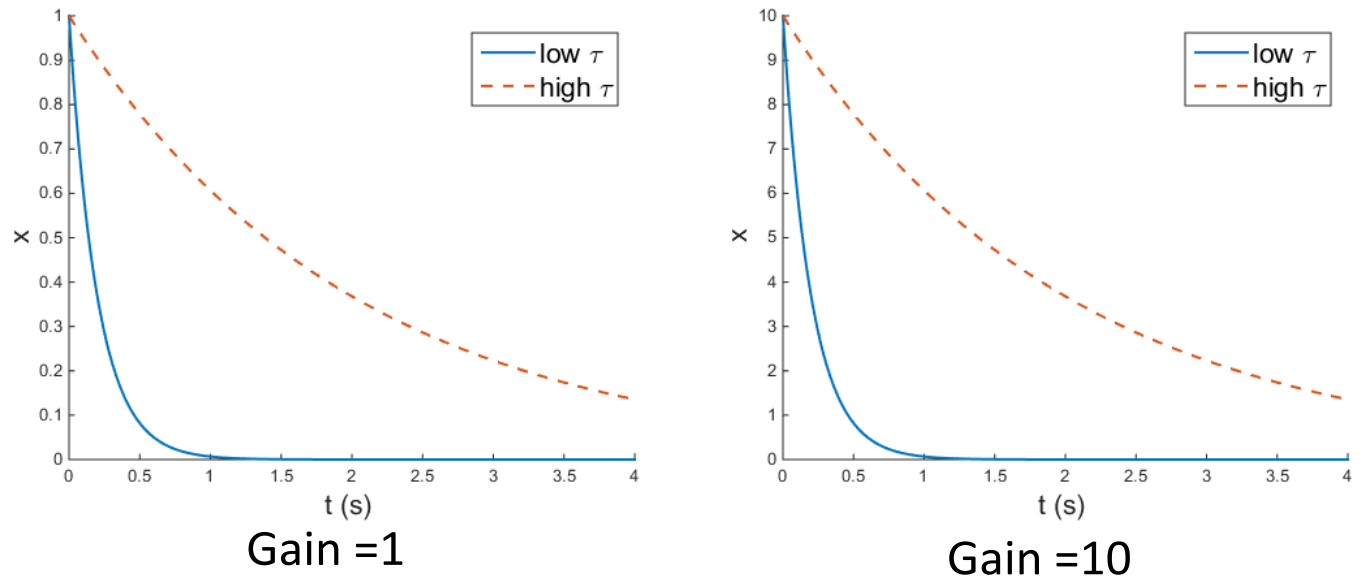
\includegraphics[width = 0.9 \textwidth]{../img/graphs6.PNG}
\end{figure}
Having a negative time constant makes no physical sense, so the exception of $T=0$, the response will always be an exponential decay.
\subsection{Unit Step Response}
\begin{figure}[H]
  \centering
  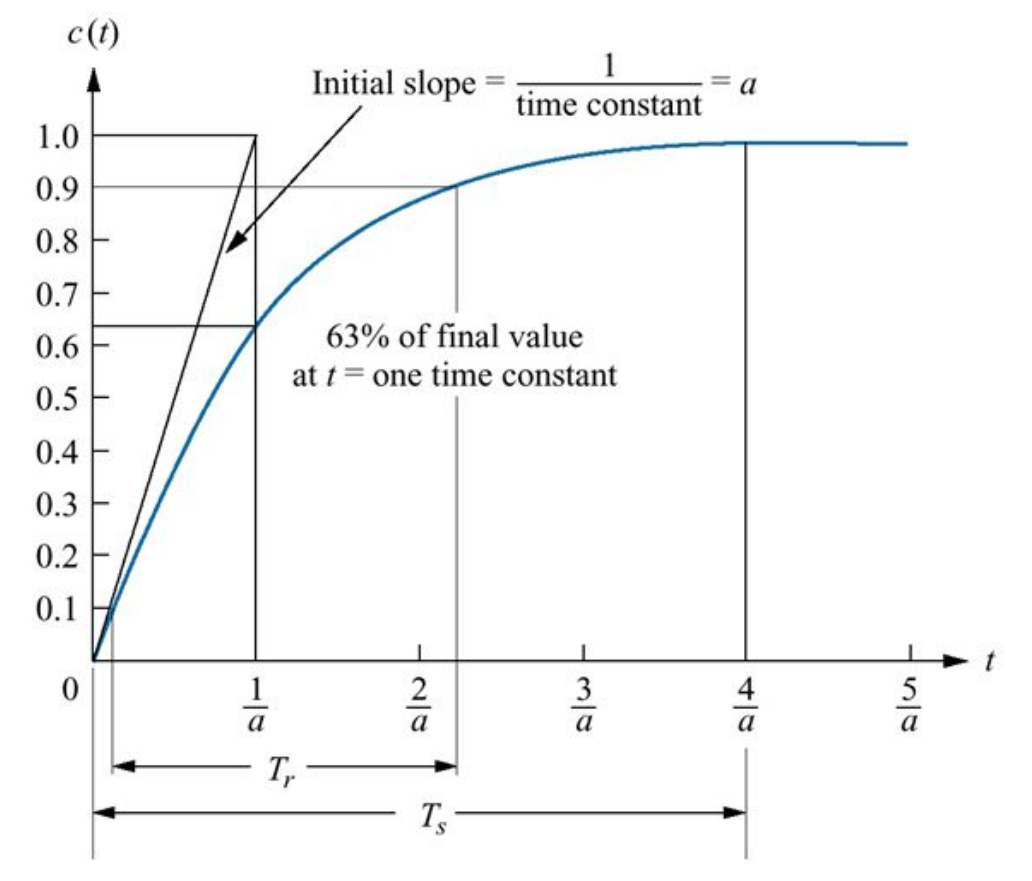
\includegraphics[width = 0.65 \textwidth]{../img/graphs7.PNG}
\end{figure}
If a step input is given to a first order system, this will result in an exponential increase. This might be something like changing the room temperature. When talking about unit step input, the amplitude of the input will vary from 0 to 1. Some important definitions are:
\begin{itemize}
  \item Initial slope = $\frac{1}{time \ constant} = a$ 
  \item $T_r =$ Raising time = how quick the exponential function achieves 90\% of the final value
  \item $\tau$ = Time constant = how quick the exponential function achieves 63\% of the final value
  \item $T_s$ = Settling time = how quick the exponential function becomes constant
\end{itemize}
Remember, we have modelled mechanical and electrical systems, and arrived at the same equations. This could be biological, financial, meteorological… This is good, because you only need to understand one system to understand hundreds. However, this means the models can appear abstract (or possibly arbitrary), so it is important to keep in mind the physical systems we are trying to model. 
\begin{figure}[H]
  \centering
  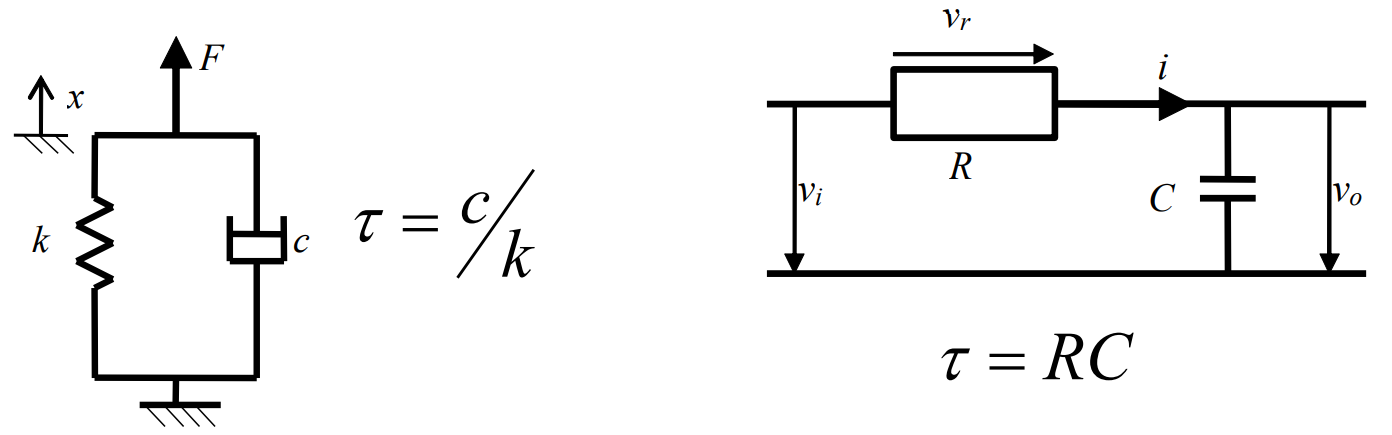
\includegraphics[width = 0.9 \textwidth]{../img/blockdiagram19.png}
  \caption{Left: Rate of decay determined by ratio of spring return force to viscous friction | Right: Rate of decay determined by total impedance of $R$ and $C$}
\end{figure}
\section{Second Order Systems}
The standard form for second order systems is shown below:
\begin{gather}
  G(s) = \gamma \frac{\omega_n^2}{s^2 + 2\zeta \omega_n s + \omega_n^2}
\end{gather}
Where:
\begin{itemize}
  \item $\gamma$ is the \textbf{gain}
  \item $\omega_n$ is the \textbf{natural frequency}
  \item $\zeta$ is the \textbf{damping ratio}
\end{itemize}
This function is known as a damped oscillator, in that it produces harmonic sinusoidal oscillations which decay over time. This type of system appears everywhere in physics, as well as in engineering. Even to the extent that some higher order systems are simplified to become second order, just because it is so well understood.
\subsubsection*{Example – Mass Spring Damper}
\begin{figure}[H]
  \centering
  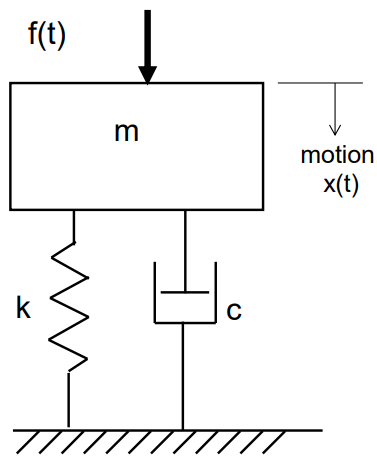
\includegraphics[width = 0.3 \textwidth]{../img/massspringdamper.PNG}
\end{figure}
Consider a simple mechanical system Mass/Spring/Damper (MSD). As before, we wish to relate the input force to the output displacement i.e. Transfer function desired:
\begin{gather}
  G(s) = \frac{X(s)}{F(s)}
\end{gather}
Balancing forces as function of time:
\begin{gather}
  f(t) = f_S(t) + f_D(t) + f_I(t)
\end{gather}
Where:
\begin{itemize}
  \item $f_S(t) = kx(t)$
  \item $f_D(t) = c\frac{\dif x(t)}{\dif t}$
  \item $f_I(t) = m\frac{\dif^2 x(t)}{\dif t^2}$
\end{itemize}
So time domain force equilibrium is:
\begin{gather}
  f(t) = kx(t) + c\frac{\dif x(t)}{\dif t} + m\frac{\dif^2 x(t)}{\dif t^2}
\end{gather}
Converting to Laplace domain:
\begin{gather}
  F(s) = kX(s) + csX(s) + ms^2X(s) \\
  F(s) = X(s)(k + cs + ms^2) \\
  G(s) = \frac{X(s)}{F(s)} = \frac{1}{ms^2 + cs + k}
\end{gather}
To obtain the Laplace domain in the "standard" form, the coefficient of the highest order of $s$ on the denominator should be 1:
\begin{gather}
  G(s) = \frac{\frac{k}{m}}{s^2 + s\frac{c}{m} + \frac{k}{m}}\frac{1}{k} \\
  = \gamma \frac{\omega_n^2}{s^2 + 2\zeta \omega_n s + \omega_n^2}
\end{gather}
Where:
\begin{itemize}
  \item $\omega_n = \sqrt{\frac{k}{m}}$
  \item $\zeta = \frac{c}{2\sqrt{km}}$
  \item $\gamma = \frac{1}{k}$
\end{itemize}
\subsection{Returning to the Time Domain}
As before, we use the inverse Laplace transform to get the time domain response. To reiterate, the benefit of standard forms is that the transforms are given in the tables:
\begin{gather}
  G(s) = \gamma \frac{\omega_n^2}{s^2 + 2\zeta \omega_n s + \omega_n^2} \\
  x(t) = L^{-1} \left\{\frac{\omega_n^2}{s^2 + 2\zeta \omega_n s + \omega_n^2} \right\} \\
  \frac{x(t)}{x(0)} = \gamma \frac{\omega_n}{\sqrt{1-\zeta^2}}e^{-\zeta \omega_n t} sin(\omega_n \sqrt{1-\zeta^2}\cdot t)
\end{gather}
$\gamma$ is not shown as it is unaffected by the Laplace transform. The equation above looks complicated, but investigating each term yields:
\begin{gather}
  \gamma \frac{\omega_n}{\sqrt{1-\zeta^2}}
\end{gather}
$\gamma \ \omega_n \ \zeta$ are all constants, so the whole term is just a number.
\begin{gather}
  e^{-\zeta \omega_n t}
\end{gather}
It is an exponential function, which depending on whether $-\zeta \omega_n$ is positive or negative, increases or decays.
\begin{gather}
  sin(\omega_n \sqrt{1-\zeta^2}\cdot t)
\end{gather}
$\omega_n \ \zeta$ are just constants, so assuming $\zeta < 1$, this is just a sine wave.
\begin{figure}[H]
  \centering
  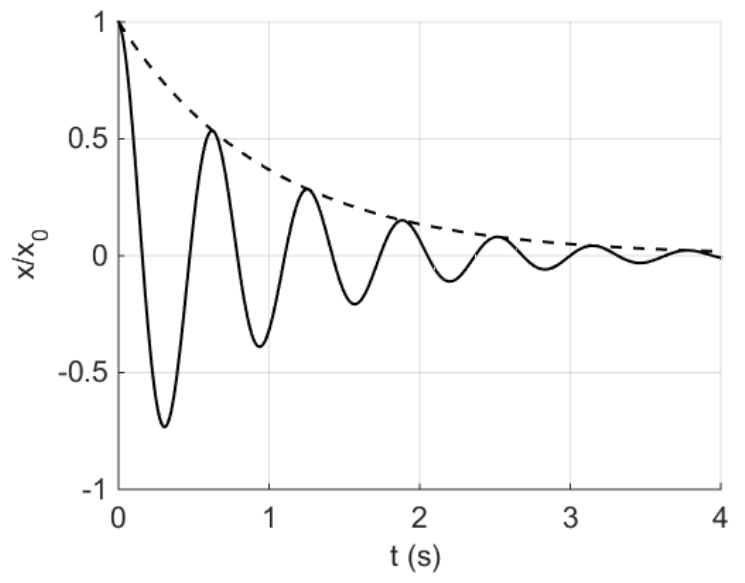
\includegraphics[width = 0.55 \textwidth]{../img/graphs8.PNG}
\end{figure}
This is an exponentially decaying sinusoidal oscillation, with:
\begin{itemize}
  \item Frequency: $\omega_n \sqrt{1-\zeta^2}\cdot t$
  \item Decay: $e^{-\zeta \omega_n t}$
  \item Gain: $\gamma \frac{\omega_n}{\sqrt{1-\zeta^2}}$
\end{itemize}
\subsection{Unit Step Response}
\begin{figure}[H]
  \centering
  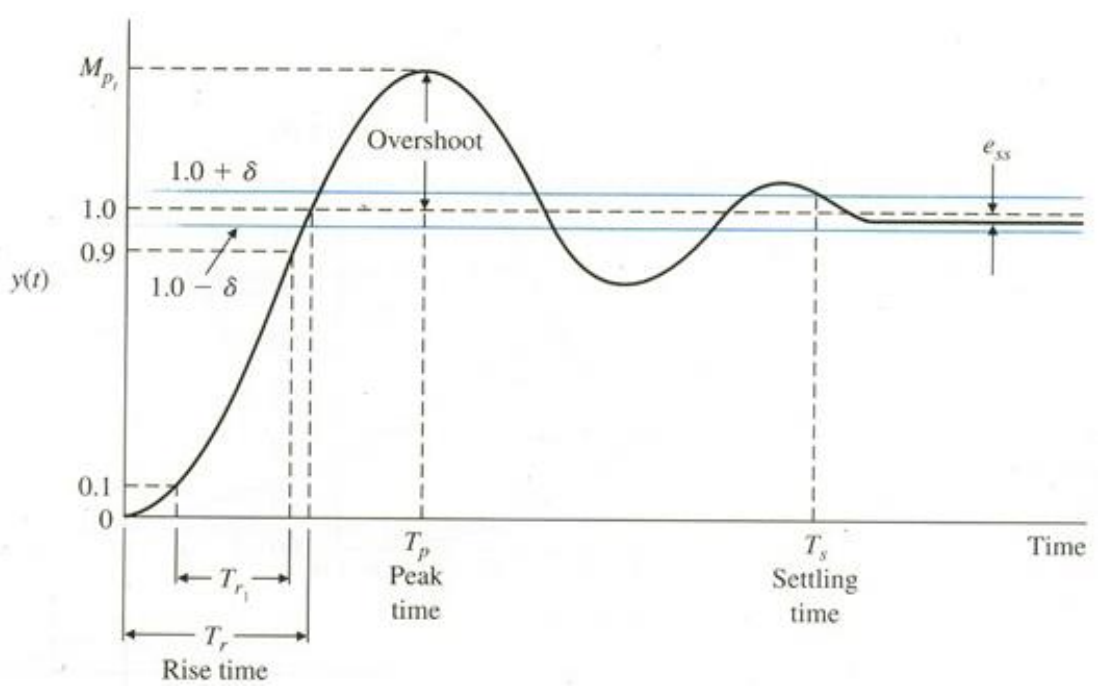
\includegraphics[width = 0.65 \textwidth]{../img/graphs9.PNG}
\end{figure}
Some properties that should be known, but will be investigated later are:
\begin{itemize}
  \item Slope at the time step input is made $(t=0)$ = 0
  \item $T_p=$ Peak Time
  \item $T_s=$ Settling Time
  \item $T_r=$ Rise Time
  \item Overshoot
\end{itemize}
\section{Tutorial}
\subsection*{LRC Filter}
\begin{figure}[H]
  \centering
  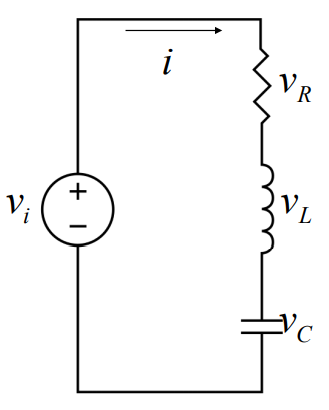
\includegraphics[width = 0.25 \textwidth]{../img/lrcfilter.PNG}
\end{figure}
A more complex filtering circuit is an LRC filter, also known as a harmonic oscillator circuit, which allows for a narrower range of frequencies to be amplified or attenuated. These circuits are used in analogue radios with a variable capacitor or inductor connected to the dial to select the frequency. To describe the relationship between the input voltage $V_i$, and the voltage across the capacitor $V_C$:
\begin{gather}
  G(s) = \frac{V_C(s)}{V_i(s)}
\end{gather}
Balancing voltages using Kirchoff's Law:
\begin{gather}
  v_i = v_R + v_L + v_C
\end{gather}
Where:
\begin{itemize}
  \item $v_r(t) = i(t)R$
  \item $v_c(t) = \frac{1}{C}\int i(t)\dif t$
  \item $v_L(t) = L\frac{\dif i(t)}{\dif t}$
\end{itemize}
So time domain voltage is:
\begin{gather}
  v_i(t) = i(t)R + \frac{1}{C}\int i(t)\dif t + L\frac{\dif i(t)}{\dif t}
\end{gather}
Converting to Laplace domain:
\begin{gather}
  V_i(s) = I(s)R + \frac{1}{Cs}I(s) + LsI(s) \\
  V_i(s) = I(s) \left(R + \frac{1}{Cs} + Ls\right)
  \label{laplacedomain1}
\end{gather}
Getting the laplace domain and rearranging the $v_c(t)$ term yields:
\begin{gather}
  v_c(t) = \frac{1}{C}\int i(t)\dif t \\
  V_c(s) = \frac{1}{Cs}I(s) \\
  I(s) = V_C(s)Cs \label{Is}
\end{gather}
Inputting equation (\ref{Is}) into equation (\ref{laplacedomain1}):
\begin{gather}
  V_i(s) = CsV_c(s) \left(R + \frac{1}{Cs} + Ls\right) \\
  G(s) = \frac{V_C(s)}{V_i(s)} = \frac{1}{LCs^2 + CRs + 1}
\end{gather}
To obtain the Laplace domain in the "standard form":
\begin{gather}
  G(s) = \frac{\frac{1}{LC}}{s^2 + s\frac{R}{L} + \frac{1}{LC}} \\
  = \frac{\omega_n^2}{s^2 + 2\zeta \omega_n s + \omega_n^2}
\end{gather}
Where:
\begin{itemize}
  \item $\omega_n = \sqrt{\frac{1}{LC}}$
  \item $\zeta = \frac{R}{2}\sqrt{\frac{C}{L}}$
  \item $\gamma = 1$
\end{itemize}


\end{document}